\documentclass[11pt,a4paper]{article}

% Note: Must use TexLive 2016 and NOT 2018 or later.
% See notes here: https://www.overleaf.com/latex/templates/acl-2020-proceedings-template/zsrkcwjptpcd

\usepackage[T1]{fontenc} 
\usepackage[utf8]{inputenc}
\usepackage[english]{babel}

\usepackage[hyperref]{acl2020}
\usepackage{times}
\usepackage{latexsym}
\renewcommand{\UrlFont}{\ttfamily\small}

% This is not strictly necessary, and may be commented out,
% but it will improve the layout of the manuscript,
% and will typically save some space.
\usepackage{microtype}

\usepackage{todonotes}
\usepackage{csquotes}
\usepackage{caption}
\usepackage{hyperref}
\usepackage{subcaption}
\usepackage{multirow}

\aclfinalcopy % Uncomment this line for the final submission

% \setlength\titlebox{5cm}
% You can expand the titlebox if you need extra space
% to show all the authors. Please do not make the titlebox
% smaller than 5cm (the original size); we will check this
% in the camera-ready version and ask you to change it back.

\newcommand\BibTeX{B\textsc{ib}\TeX}

\title{Speech2Text in JoeyNMT}

\author{\small Stefan Machmeier \\
  \small Department of Computer Science \\
  \small Heidelberg University, Germany \\
  \small \textit{tz251@stud.uni-heidelberg.de} \\
  \And
  \small Robin Fleige \\
  \small Department of Computer Science \\
  \small Heidelberg University, Germany \\
  \small \textit{lq250@stud.uni-heidelberg.de} \\
  \And
  \small Andre Meyering \\
  \small Department of Computer Science \\
  \small Heidelberg University, Germany \\
  \small \textit{hp250@stud.uni-heidelberg.de} \\}

\date{\today}

\begin{document}
\maketitle
\begin{abstract}
In this paper we are looking into speech to text transformations using the JoeyNMT neural machine translation toolkit.
We adapt JoeyNMT's existing code base to additionally handle audio files.
We achieve this by including Torchaudio, the audio counterpart of the Torchtext project which is heavily used by JoeyNMT.
\todo{Nicht vollständig}
\end{abstract}

\section{Introduction}

JoeyNMT is an open source project for neural machine
translation (NMT) that aims to be easy to understand while implementing modern approaches. This gives beginners the possibility to quickly and easily understand the architecture and customize individual parts to experiment with the behavior.
In this thesis the possibility to use JoeyNMT for processing speech to text is worked out. For this purpose, the Mel Frequency Cepstral Coefficients (MFCC) of the audio files is used as input for JoeyNMT. As datasets we use audio from the common voice project, where it is possible to filter by language, accent and quality, so that uniform data can be used.

\section{Related Work}

Speech to text transformations are common but in context of JoeyNMT, we found that it references one project that does this.
\enquote{Speech Joey}\cite{speech_joey} extends JoeyNMT with functionality for speech recognition and is written by Sariya Karimova\footnote{See \url{https://www.cl.uni-heidelberg.de/~karimova/}, last visited 2021-09-09}, a former graduate research assistant at the Statistical NLP group of the Heidelberg University.
However, the project does not run anymore due to breaking changes in the project's
dependencies and missing versions in their list of dependencies.
Furthermore, after trying to install older versions of certain dependencies,
we noticed that some were not available for more recent versions of Python such as 3.8 or 3.9.
We still looked at the project as it was listed by JoeyNMT itself.
In comparison to our project, Speech Joey uses \enquote{librosa}\footnote{See \url{https://librosa.org/doc/latest/index.html}, lasted visited 2021-09-09} whereas we use Torchaudio.
The underlying transformations should still be very similar but we were unable to compare our results against Speech Joey.


\section{JoeyNMT}

\todo{Was zu JoeyNMT schreiben? Oder aus der Einleitung was raus nehmen?}

\section{Speech To Text}

\todo{Grundsätzlich was zu speech2text schreiben.}

\subsection{Feature Extraction}

As audio files are just binary blobs and cannot be worked with as text,
we cannot work with JoeyNMT's existing feature extractions for text.

For audio processing, there are multiple common ways to represent audio signals.
One common visualization is the waveform representation as can be seen in \autoref{fig:1021_waveform}.
The figure visualizes amplitude changes over time.
Its benefit lies in the detection audio detection, where values near zero indicate silent sounds and larger amplitudes indicate louder sounds.
It can be used to detect pauses between spoken words and it is possible to detect voiced and unvoiced sounds and even certain vowels can be detected~\cite{Comer_1162014}.

Another way to visualize audio signals are Spectrograms, as can be seen in \autoref{fig:1021_spectrogramm}.
The waveform is visualized as a Spectrogram and shows more details of the audio signals, or rather, it shows the spectrum of frequencies over time.
Oftentimes, the Mel frequency spectrum is used~\cite{MelFreq} as this represents the human audio perception.

However, there are further frequency transformations of audio signals
that can be used to translate spoken to written words.

According to Wang and Lawlor, \enquote{MFCC is one of more the successful methods} for speech to text systems which is \enquote{based on the human peripheral auditory system}~\cite{Wang_7983644}.
Therefore, MFCC (short for Mel Frequency Cepstral Coefficients) is another transformation that yields good results for speech recognition.
\autoref{fig:1021_mfcc} shows the resulting Spectrogram after applying MFCC.
We note that there are possibilities to improve results even more, as described in \cite{Winursito_8350748}.

We refer to \cite{ittichaichareon2012speech} and \cite{singh2014approach} for a detailed description of MFCC.
 
\begin{figure*}[htb]
    \begin{subfigure}[b]{0.32\textwidth}
        \centering
        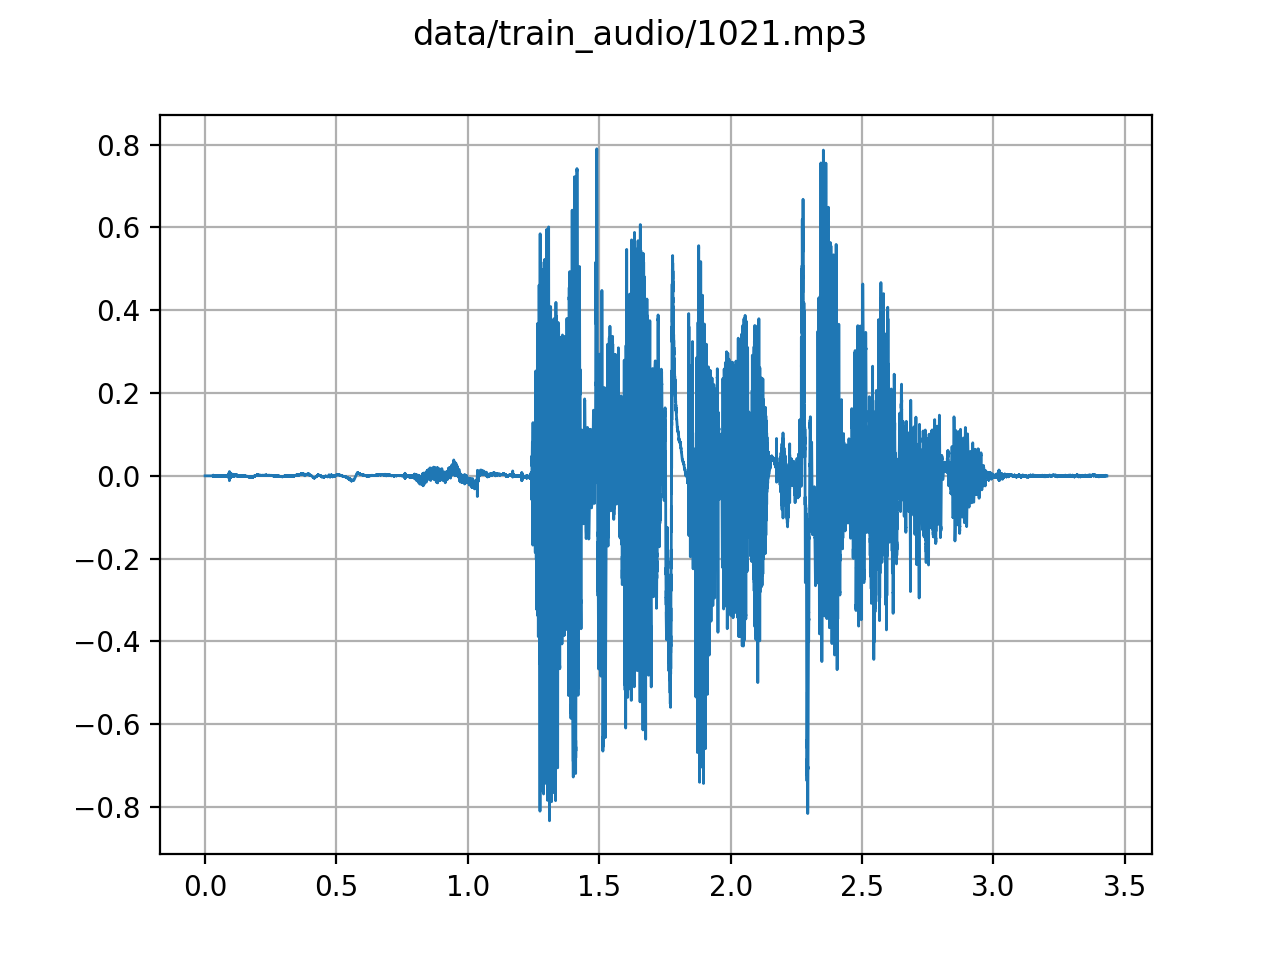
\includegraphics[width=\textwidth]{joeynmt-speech2text/images/1021_Eine_Beleuchtung_ist_vorgeschrieben_Waveform.png}
        \caption{Waveform}
        \label{fig:1021_waveform}
    \end{subfigure}
     \hfill
    \begin{subfigure}[b]{0.32\textwidth}
        \centering
        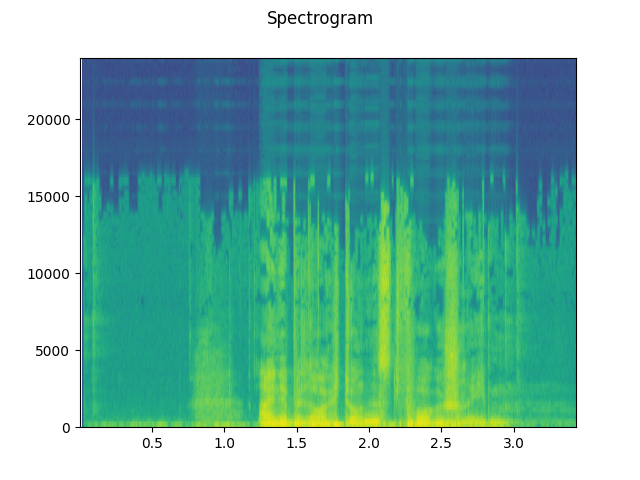
\includegraphics[width=\textwidth]{joeynmt-speech2text/images/1021_Eine_Beleuchtung_ist_vorgeschrieben_Spectrogram.png}
        \caption{Spectrogramm}
        \label{fig:1021_spectrogramm}
    \end{subfigure}
     \hfill
    \begin{subfigure}[b]{0.32\textwidth}
        \centering
        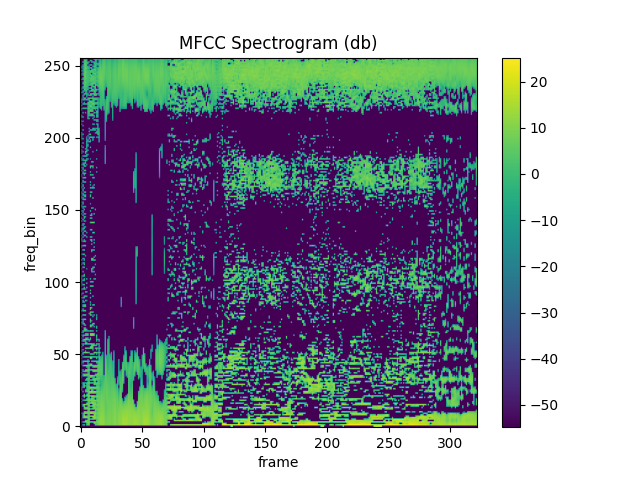
\includegraphics[width=\textwidth]{joeynmt-speech2text/images/1021_Eine_Beleuchtung_ist_vorgeschrieben_MFCC.png}
        \caption{MFCC}
        \label{fig:1021_mfcc}
    \end{subfigure}
    \caption{Visualizations of \enquote{Eine Beleuchtung ist vorgeschrieben.}}
    \label{fig:beleuchtung_viz}
\end{figure*}

\subsection{Dataset}
\label{subsec:dataset}

The dataset used throughout this paper is the open \enquote{Common Voice Corpus 7.0} dataset by Mozilla~\cite{commonvoice:2020}.
We have chosen the German language as that's what the authors are most familiar with which allows us to better evaluate the dataset quality.
The unprocessed dataset contains 26\,GB of audio files which 1035\,h according to \enquote{Common Voice}.

After listening to few audio files, the authors decided to filter the dataset for one major reason:
There were audio files that had accents that made it hard to understand even for native speakers.

Furthermore, even though the authors think that enterprise speech to text models
should handle accents as well as differences between male and female voices,
we decided that it would be out-of-scope for this paper.
Therefore, all audio files were filtered according to these rules:

\begin{itemize}
    \item max. 75 characters
    \item no accent and no Swiss- or Austrian-German
    \item male voice
    \item no special characters in the corresponding text\newline 
          this include punctuation such as \texttt{.,!?} and quotation marks
    \item lowercasing characters in the corresponding texts
\end{itemize}

Having these limitations makes it easier to rule out issues during evaluation.

However, these limitations yield only about 7500 audio files for training and around 100 for testing and evaluation.  On top of this, the quality of audio files still differs enormously.  Whereas some have crystal clear voices, other have lot of noise and even contain mouse-click or keyboard sounds.


\section{Results and Discussion}

We compared two different models. \autoref{tab:parameters} lists all important hyperparameters. As a basis we chose the default JoeyNMT configuration, and adapted the hidden size, and layers for decoder and encoder. As previously mention, we limited our self to MFCC only. Each model will be compared by the best validation perplexity (ppl) that have been achieved during training. Perplexity is a exponentiation of the entropy, and it tells us how well our natural language model predicts test data. A lower perplexity indicates a good prediction whereas a high perplexity indicates the opposite \cite{jozefowicz2016exploring}

\begin{table}[]
\centering
\caption{Hyperparameters of both models. We only listed the most important ones.}
\begin{tabular}{ll|l|l}
                         & Hyperparameter & Model A  & Model B \\\hline
                         & RNN type       & LSTM     & LSTM    \\
                         & Learning rate  & $0.001$  & $0.001$ \\
                         & level          & char     & char    \\
                         & scheduling     & plateau  & plateau \\
                         & epochs         & $30$     & $30$      \\\hline
\multirow{3}{*}{Encoder} & layers         & $8$      & $8$       \\
                         & hidden size    & $64$     & $64$      \\
                         & dropout        & $0.1$    & $0.2$     \\\hline
\multirow{5}{*}{Decoder} & layers         & $8$      & $8$       \\
                         & hidden size    & $256$    & $512$     \\
                         & dropout        & $0.1$    & $0.2$     \\
                         & hidden dropout & $0.1$    & $0.2$     \\
                         & attention      & luong    & bahdanau\\    
\end{tabular}
\label{tab:parameters}
\end{table}

Both models were trained on the same preprocessed dataset that has been described in \autoref{subsec:dataset}. Our idea was to have a basis that we try to improve by fine-tuning our hyperparameters. Specifically, we choose dropout, attention, and hidden size for model B. \autoref{tab:results} shows the achieved results. The first model reached . Increasing the hidden size of model b lead to 

\begin{table}[]
    \centering
    \caption{Results}
    \begin{tabular}{c|c}
        Model & Perplexity\\
        \hline
        A     &  \\
        B     & 
    \end{tabular}
    
    \label{tab:results}
\end{table}

%\begin{figure*}
%    \centering
%    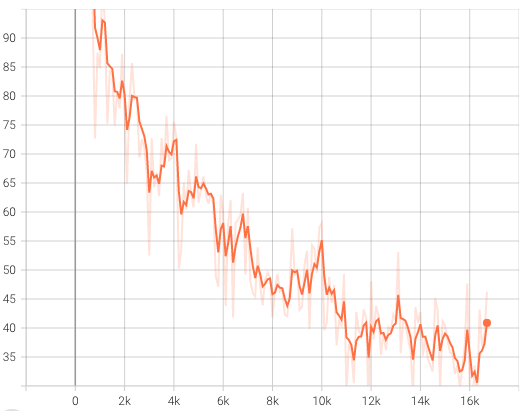
\includegraphics[width=\textwidth]{joeynmt-speech2text/images/train_loss.png}
%    \caption{Training loss over 30 epochs. The orange line is the loss for the training set.}
%    \label{fig:train_loss}
%\end{figure*}

%\begin{figure*}
%    \centering
%    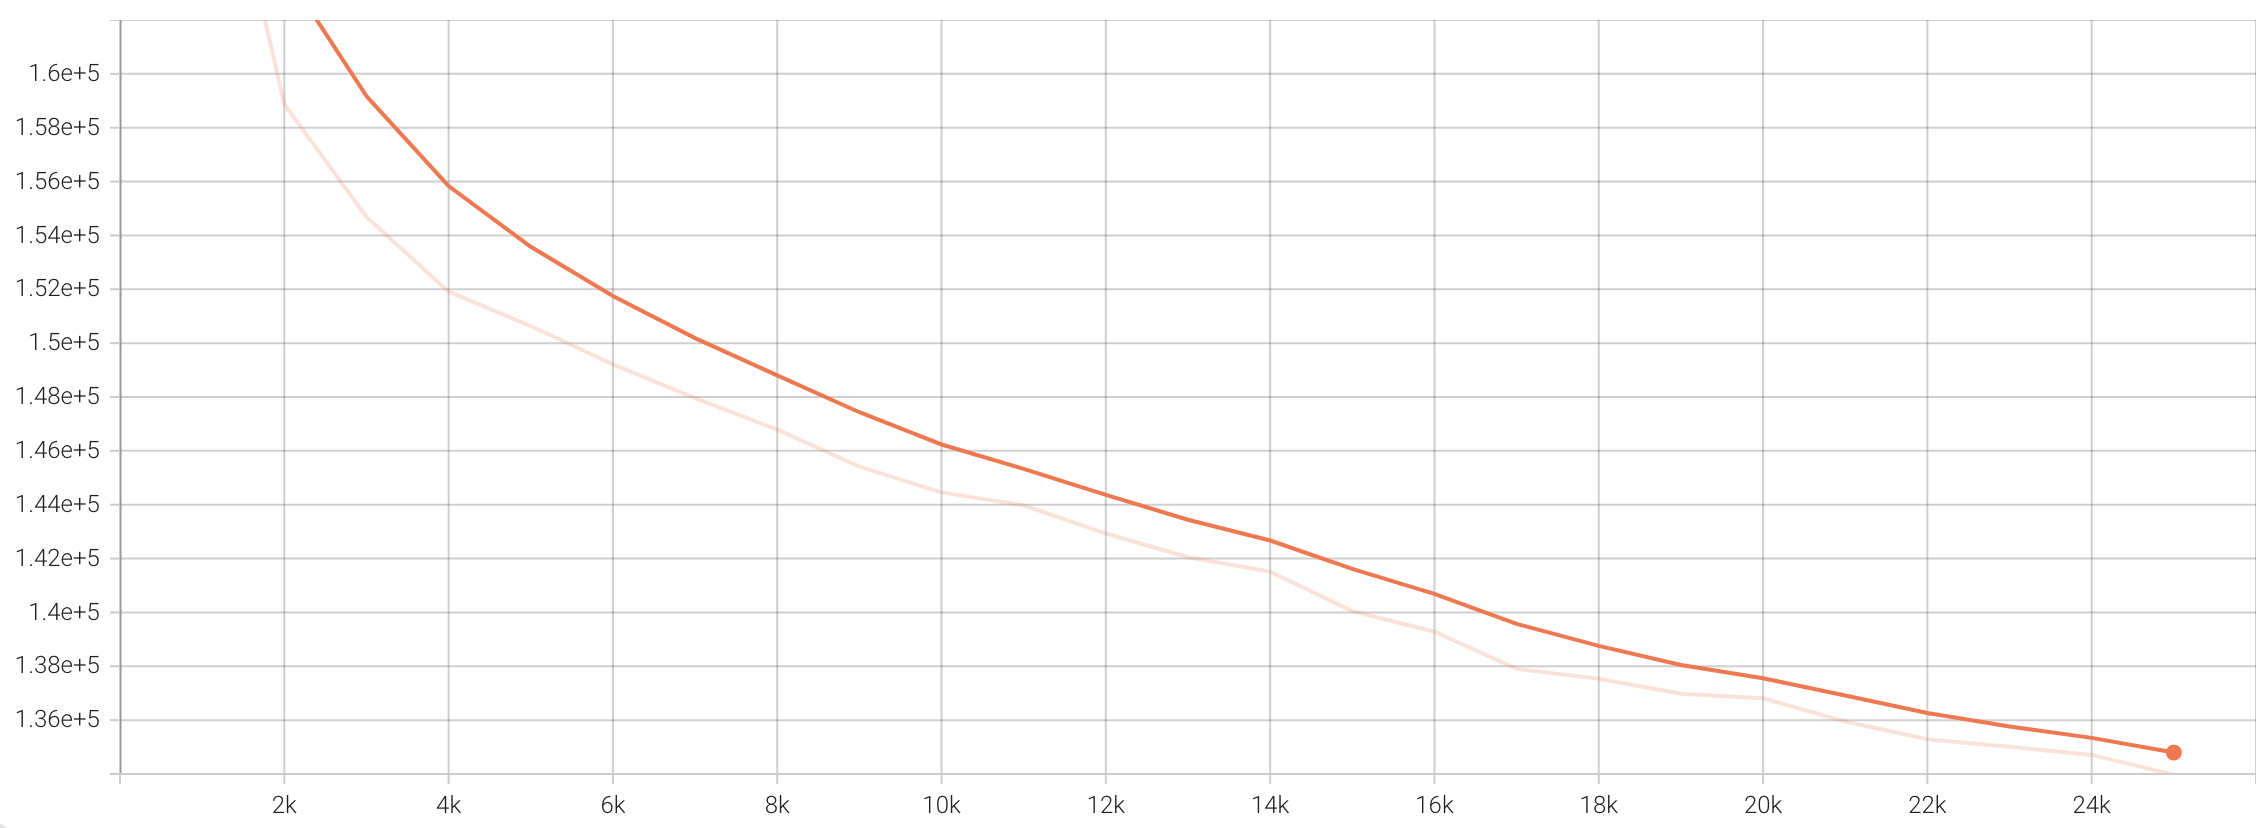
\includegraphics[width=\textwidth]{joeynmt-speech2text/images/val_loss.png}
%    \caption{Test loss over 30 epochs. The orange line is the loss for the test set.}
%    \label{fig:val_loss}
%\end{figure*}

\bibliography{acl2020}
\bibliographystyle{acl_natbib}

\appendix

\section{Appendices}
TODO

\section{Supplemental Material}
\label{sec:supplemental}
TODO

\end{document}
